% !TeX root = ../../tesi.tex

The depth sensing module of the Microsoft Azure Kinect DK is based on the Time-of-Flight (ToF) principle, a technique used to estimate the distance between the sensor and objects in the scene by measuring the time required for emitted light to travel to the target and back to the sensor.
\begin{figure}[h]
    \centering
    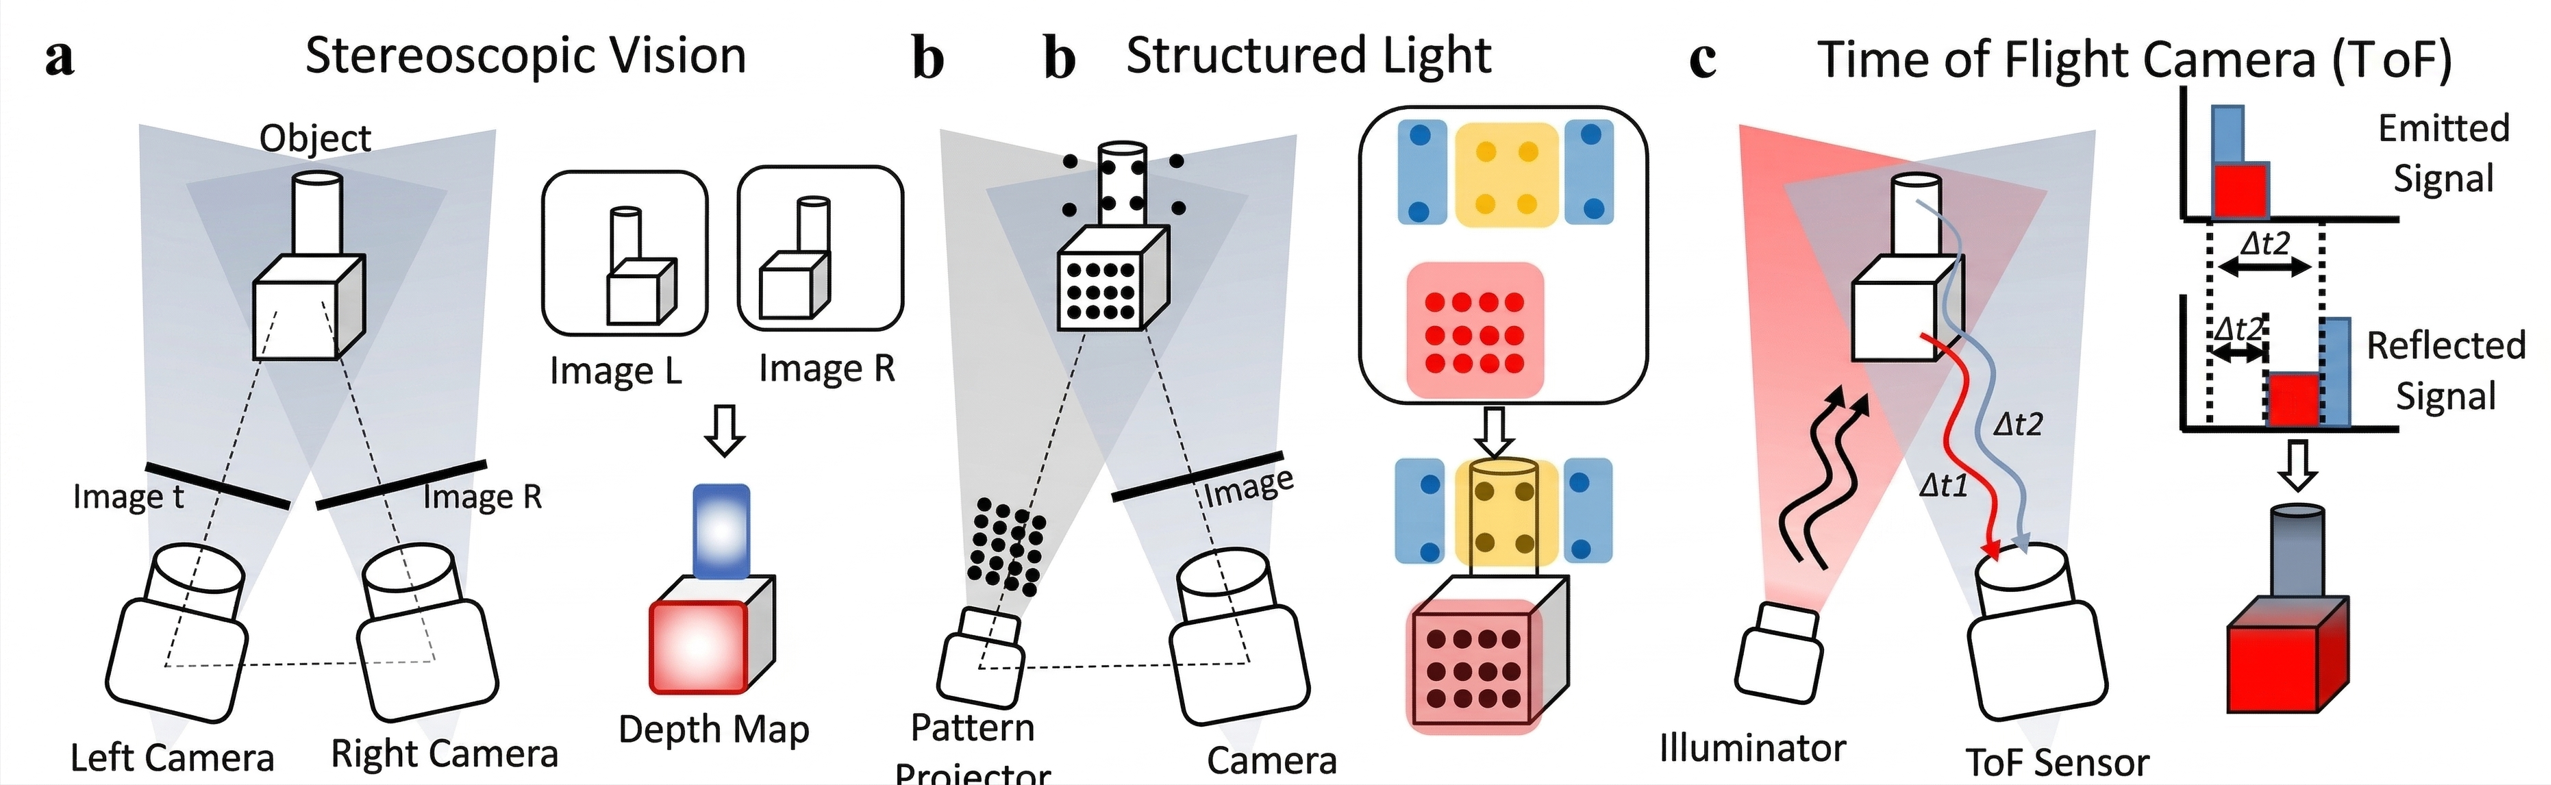
\includegraphics[width=0.7\linewidth]{images/ToF.png}
    \caption{Different depth estimation approaches}
    \label{fig:Depth}
\end{figure}

In general, the depth $Z$ of a point can be computed as:

\begin{equation}
Z = \frac{c \cdot \Delta t}{2}
\end{equation}

where:
\begin{itemize}
    \item $c$ is the speed of light in air,
    \item $\Delta t$ is the round-trip travel time of the emitted optical signal.
    \item The division by two accounts for the two-way propagation path (sensor-to-object and object-to-sensor).
\end{itemize}

Direct measurement of $\Delta t$ requires extremely high temporal resolution, as light travels approximately 30~cm in 1~ns. For this reason, most modern ToF cameras, including the Azure Kinect, employ a \textit{continuous-wave modulation} approach rather than direct pulsed time measurement.

\begin{figure}[h]
    \centering
    \includegraphics[width=0.5\linewidth]{images/ToF_pulse_vs_cont.jpg}
    \caption{Different ToF approaches}
    \label{fig:ToF_1}
\end{figure}

In continuous-wave ToF systems, the emitted infrared light is amplitude-modulated at a known frequency. The reflected signal received by the sensor exhibits a phase shift $\phi$ proportional to the propagation delay. The depth is then computed as:

\begin{equation}
Z = \frac{c}{4\pi f} \phi
\end{equation}

where:
\begin{itemize}
    \item $f$ is the modulation frequency,
    \item $\phi$ is the measured phase difference between emitted and received signals.
\end{itemize}

\begin{figure}[h]
    \centering
    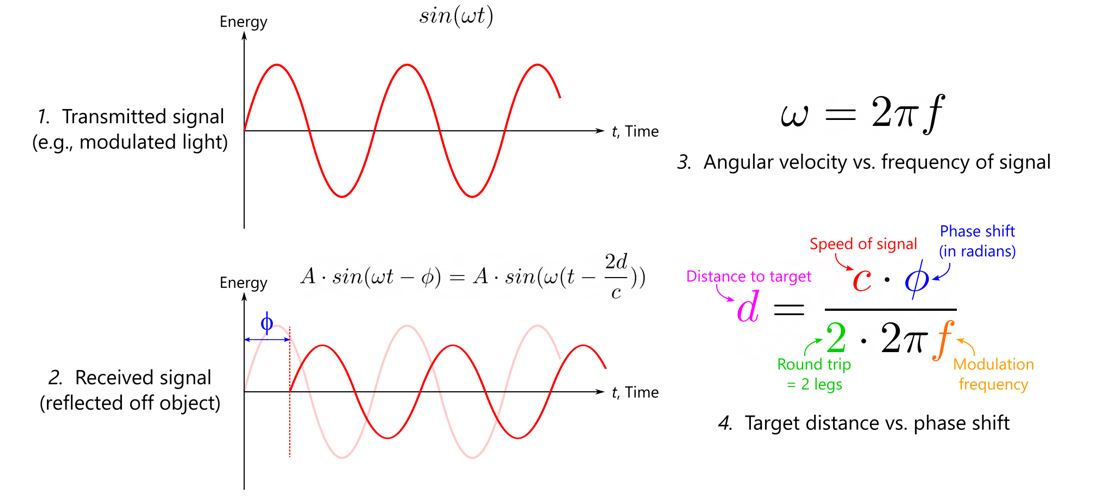
\includegraphics[width=0.7\linewidth]{images/ToF_1.jpg}
    \caption{Time of flight equations derivation}
    \label{fig:ToF_2}
\end{figure}

By estimating the phase shift at each pixel, the sensor generates a dense depth map, enabling per-pixel 3D reconstruction of the observed scene.
\\
The advantages of ToF-based depth sensing include:
\begin{itemize}
    \item direct acquisition of metric depth measurements,
    \item dense depth maps without requiring stereo matching,
    \item robustness to moderate textureless surfaces.
\end{itemize}

However, ToF systems are subject to several sources of error, including:
\begin{itemize}
    \item multipath interference (MPI), caused by indirect reflections,
    \item ambient infrared light interference,
    \item phase ambiguity at larger distances due to periodic modulation,
    \item reduced accuracy on highly reflective or absorptive materials.
\end{itemize}

Despite these limitations, Time-of-Flight technology provides accurate and dense depth measurements in indoor environments, making it particularly suitable for volumetric estimation and 3D reconstruction tasks, as required in the present application.
